\chapter{Mejora del hardware de los electroestimuladores}
El presente capítulo se centra en el estudio y mejora del hardware de los estimuladores eléctricos de la prótesis híbrida. Se plantea este capítulo con el objetivo principal de obtener un electroestimulador robusto, ligero y de tamaño reducido.
\\
\\
Se identificará en primer lugar el conjunto de objetivos de mejora del mencionado dispositivo que servirán de guía para el planteamiento de tareas enfocadas a mejorar su hardware. 
\\
\\
Por último, se expondrá el cumplimiento de dichas tareas así como la validación de objetivos para mostrar en efecto una mejora en el hardware del electroestimulador.

\section{Etapa de potencia}\label{mejora_hardware_potencia}
La etapa de potencia del electroestimulador es la que más trabajo necesita en cuanto a tareas de mejora. Se va a explicar en este apartado el conjunto de características de la misma así como los motivos para efectuar una mejora sustancial en ésta. 

\subsection{Revisión del hardware y planteamiento de objetivos de mejora}
Tal y como se explicó en el estudio de la prótesis híbrida realizado en el apartado \ref{etapa_potencia} del capítulo \ref{capitulo_2}, la etapa de potencia del electroestimulador pertenece a una versión anterior del mismo llamada TEREFES. Esta etapa reciclada dispone de los siguientes elementos los cuales se pueden ver en la figura \ref{fig:fuente_terefes}:

\begin{itemize}
\item[•] Entrada de $5Vdc$ desde una batería externa.
\item[•] Una fuente de $5Vdc$ implementada con un convertidor de corriente continua. Su entrada son los $5Vdc$ de la batería y su salida son $5Vdc$. Además, se utilizan diferentes componentes pasivos.
\item[•] Dos fuentes de $15Vdc$ y $\pm15Vdc$ implementadas con dos convertidores de corriente continua de $5Vdc$ a $15Vdc$ y $5Vdc$ a $\pm15Vdc$ respectivamente. Se tienen también diferentes componentes pasivos. La entrada de $5Vdc$ de los convertidores procede de la batería.
\end{itemize}

Sin embargo, el electroestimulador utilizado en la prótesis híbrida no necesita una de las fuentes de $15Vdc$ y $\pm15Vdc$ lo cual se aprecia en la figura \ref{fig:fuente_mini_terefes}. Esto implica que el montaje de la etapa de potencia del mini TEREFES requiere recortar una de las placas de circuito impreso de la etapa de potencia del TEREFES de la forma mostrada en la figura \ref{fig:potencia_recorte}. En esta figura, el cable negro superior conecta las masas de los recortes de la placa mientras que el cable rojo superior conecta su alimentación de $5Vdc$ desde una batería externa. Los cables rojo y negro inferiores sirven para el encendido y apagado del convertidor de $\pm15Vdc$ desde el microcontrolador de la etapa de control. 
\\
\\
Por otra parte, las salidas de las fuentes de tensión alimentan la etapa de control mediante cables del tipo ``jumper'' que conectan los correspondientes puntos de ambas placas mediante pines montados ``through hole''. Dichos pines son los que llevan los niveles de tensión mencionados previamente así como las referencias de masa de cada fuente. De este modo, la fuente de $5Vdc$ tiene dos pines a su salida, los $5Vdc$ y su referencia a masa. La fuente de $15Vdc$ dispone así mismo de dos pines en su salida, el que aporta el nivel de tensión mencionado y la referencia a masa. Por último, la fuente de $\pm15Vdc$ tiene tres pines en su salida y que corresponden a los niveles de tensión de $15Vdc$, $-15Vdc$ y su referencia a masa. Tanto el montaje de las tarjetas de control y potencia como su conexión eléctrica se muestra en las figuras \ref{fig:etapas} y \ref{fig:placas}.
\\
\\
Además, el tamaño de la tarjeta de la etapa de potencia no es todo lo compacta posible debido a su procedencia. En un aplicación como en la que se involucra el presente Trabajo Fin de Máster, el tamaño y por tanto peso y volumen de los componentes de la prótesis híbrida es un factor de vital importancia. Se pretende llevar a cabo un asistencia al paciente de la forma menos invasiva posible. En este caso, se desea reducir el tamaño de la etapa de potencia y por tanto del estimulador eléctrico ya que el paciente llevará puestos hasta cuatro de estos dispositivos.\\

\begin{figure}[!htb]
\minipage{0.45\textwidth}
  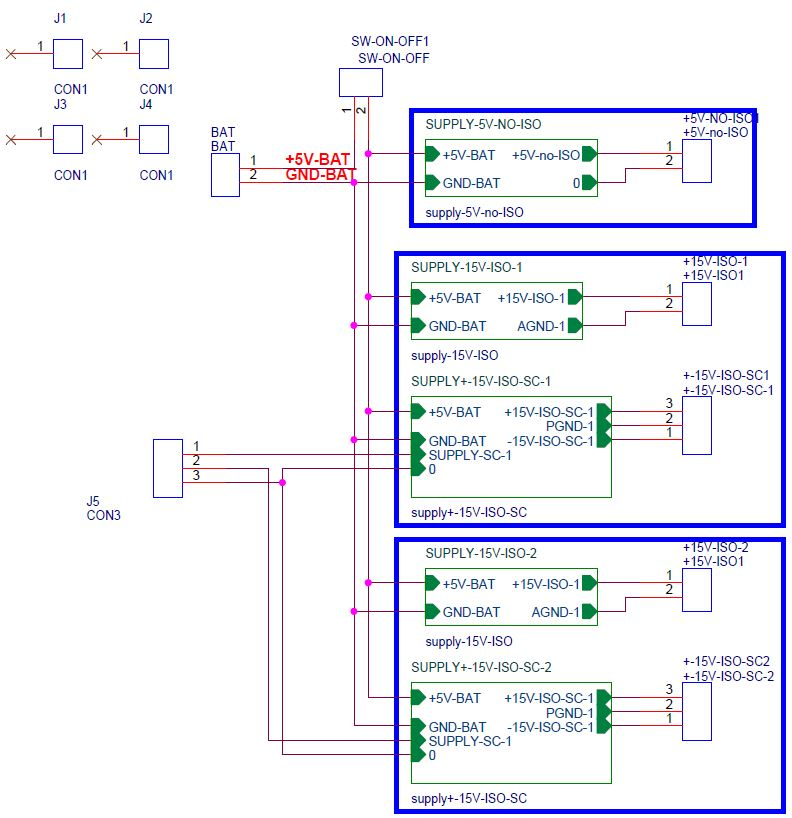
\includegraphics[width=\linewidth]{fuente_terefes}
  \caption{Esquemático de la etapa de potencia del TEREFES con alimentación a $5Vdc$ de la batería (BAT), una fuente de $5Vdc$ en cuadro el azul superior y dos fuentes de $15Vdc$ y $\pm15Vdc$, cada una de ellas en los dos cuadros azules inferiores.}\label{fig:fuente_terefes}
\endminipage\hfill
\minipage{0.45\textwidth}
  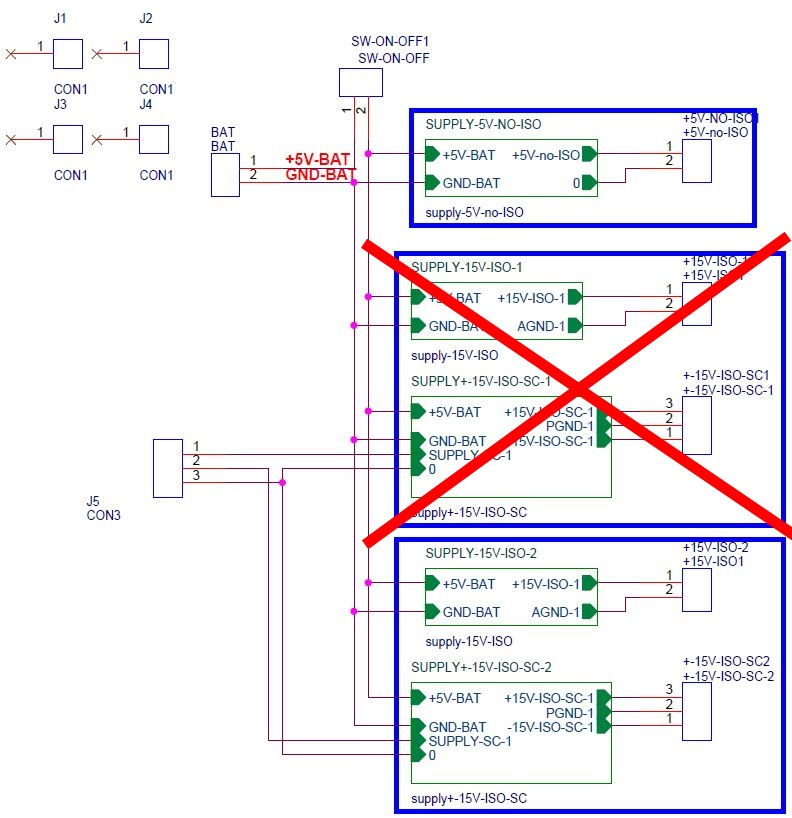
\includegraphics[width=\linewidth]{fuente_mini_terefes}
  \caption{Esquemático de la etapa de potencia del mini TEREFES con una fuente de $5Vdc$ y otra de $15Vdc$ y $\pm15Vdc$.}\label{fig:fuente_mini_terefes}
\endminipage\hfill
\end{figure}

\begin{figure}[!htb]
\centering
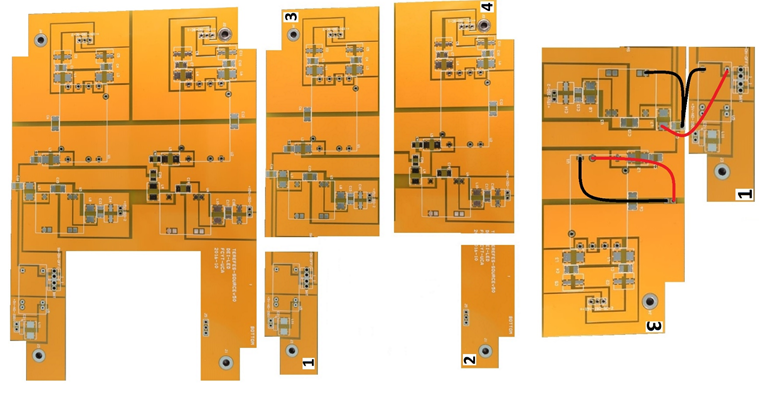
\includegraphics[scale=0.7]{potencia_recorte}
  \caption{Adapatación de la etapa de potencia reciclada del estimulador TEREFES. A la izquierda se tiene la etapa de potencia original. En el centro se muestran los cortes efectuados y los bloques resultantes numerados. A la derecha se conectan los bloques 1 y 3 necesarios para la etapa de potencia del mini TEREFES que contienen la fuente de $5Vdc$ y las fuente de $15Vdc$ y $\pm15Vdc$ respectivamente.}\label{fig:potencia_recorte}
\end{figure}

\begin{figure}[!htb]
\minipage{0.5\textwidth}
  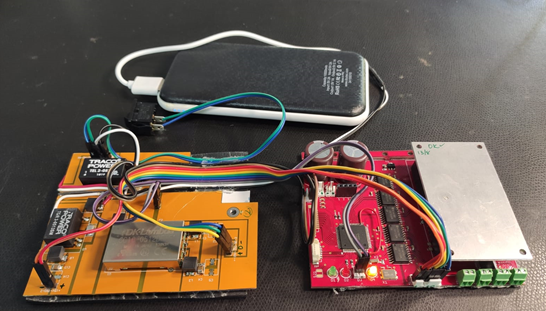
\includegraphics[width=\linewidth]{etapas}
  \caption{Etapas de control (placa roja) y de potencia (placa naranja) junto a la batería portátil que alimenta el estimulador. Los cables que conectan la placa de potencia con la de control proporcionan los niveles de tensión de $5Vdc$, $15Vdc$ y $\pm15Vdc$.}\label{fig:etapas}
\endminipage\hfill
\minipage{0.4\textwidth}
  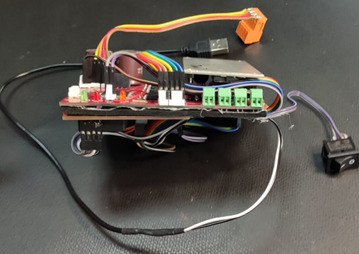
\includegraphics[width=\linewidth]{placas}
  \caption{Montaje enfrentado de las etapas de control y potencia.}\label{fig:placas}
\endminipage\hfill
\end{figure}

Se identifica en este punto un problema de tamaño e integridad de la etapa de potencia del mini TEREFES ya que se está utilizando una tarjeta de circuito impreso que no ha sido diseñada específicamente para este electroestimulador. Además, las placas de potencia y control están unidas eléctricamente mediante jumpers, los cuales no son ideales en conexiones que deben ser fiables. Es más, el estimulador va sujeto en el paciente durante ejercicios de rehabilitación que implican movimiento y manipulación del dispositivo para su puesta a punto y correcta colocación. 
\\
\\
Por lo tanto, aunque el dispositivo es funcional existen vías de mejora en cuanto a su etapa de potencia. De este modo, una vez comprendido el estado del mini TEREFES en cuanto a dicha etapa, se plantea el rediseño de la misma de modo que se fijan los siguientes objetivos:

\begin{itemize}
\item[\textbf{1)}] Reducción y optimización del tamaño y forma de la tarjeta de circuito impreso de la etapa de potencia. Ésta se adaptará al tamaño y forma de la tarjeta de control.
\item[\textbf{2)}] Alineamiento de las salidas de las fuentes de tensión de la etapa de potencia con los puntos de la etapa de control que requieren esta alimentación. Se parte del la idea de que el montaje de las placas de control y potencia se efectúa enfrentando sus reversos según se muestra en la figura \ref{fig:placas}. Se pretende entonces situar las salidas de los convertidores en la placa de potencia de manera que al efectuar el montaje mencionado previamente, queden alineadas con los puntos de la placa de control que necesitan esta alimentación. Esta conexión es posible porque tanto las salidas de las fuentes de la placa de potencia como los puntos de la placa de control que conectan con los anteriores, son agujeros en sus tarjetas de circuito impreso correspondientes. Esto implica que dichos puntos se pueden conectar mediante pines soldados a los agujeros mencionados. Se explica en las figuras \ref{fig:montaje_alineado} y \ref{fig:montaje_alineado_seccion} este objetivo.\\

\begin{figure}[!htb]
\centering
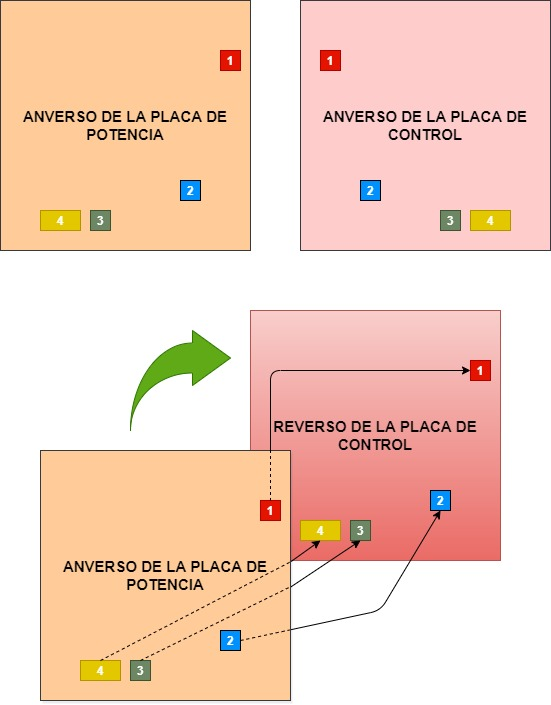
\includegraphics[scale=0.5]{montaje_alineado}
  \caption{Representación del montaje alineado de las placas de potencia y control. En la parte superior se disponen ambas placas por su anverso. En la parte inferior se ha volteado horizontalmente la placa de control y se coloca sobre ésta la placa de potencia, de modo que los reversos quedan enfrentados. Los cuadros 1, 2, 3 y 4 son las conexiones de ambas placas que se desean alinear: la conexión 1 es la salida de $5Vdc$ del correspondiente convertidor de la etapa de potencia y el punto que requiere esta tensión en la placa de control. La conexión 2 es el control remoto para el encendido y apagado del convertidor de $\pm15Vdc$ efectuado desde el microcontrolador de la placa de control. Por último, las conexiones 3 y 4 son las salidas de los convertidores de $15Vdc$ y $\pm15Vdc$ respectivamente y que aportan este nivel de tensión a los correspondientes puntos de la placa de control. Las conexiones 1, 2 y 3 necesitan dos pines mientras que la 4 necesita tres, tal y como se ha explicado con aterioridad.}\label{fig:montaje_alineado}
\end{figure}

\begin{figure}[!htb]
\centering
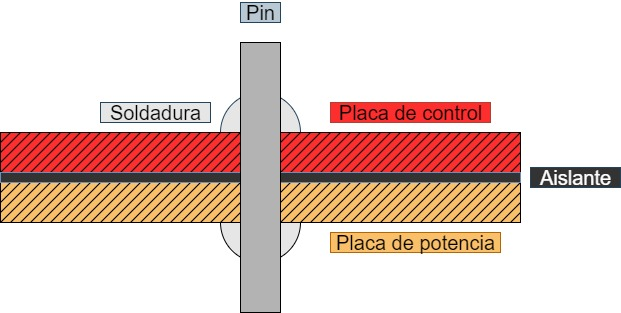
\includegraphics[scale=0.5]{montaje_alineado_seccion}
  \caption{Representación de la sección del montaje alineado de las placas del mini TEREFES. El pin representa la unión soldada de las placas entre los puntos correspondientes de las placas de control y potencia.}\label{fig:montaje_alineado_seccion}
\end{figure}

\end{itemize}

\subsection{Rediseño de la etapa de potencia}
La mejora de la etapa de potencia del mini TEREFES se realiza con Eagle\cite{eagle}, un software de diseño asistido por computador para la realización de esquemáticos de circuitos electrónicos y tarjetas de circuito impreso. Se ha elegido este software debido a que la etapa de control del electroestimulador se ha creado con el mismo, de modo que el principal motivo para dicha elección es la homogeneidad en diseños electrónicos de este componente de la prótesis híbrida. Además, el autor del presente trabajo dispone de licencia de estudiante de Autodesk, compañía propietaria de Eagle.

\subsubsection{Esquemático}
Se parte del diseño original de la etapa de potencia, es decir del TEREFES, dispositivo del que procede el estimulador eléctrico de la prótesis híbrida, el mini TEREFES. Este diseño, tal y como se ha descrito con anterioridad, dispone de una entrada de $5Vdc$ desde una batería externa, una fuente de $5Vdc$ y dos fuentes de $15Vdc$ y $\pm15Vdc$. En la figura \ref{fig:fuente_terefes} mostrada anteriormente se aprecia un esquemático a alto nivel de esta etapa mientras que en las figuras \ref{fig:fuente5vdc_esquematico}, \ref{fig:fuente15vdc_esquematico} y \ref{fig:fuente+-15vdc_esquematico} del Anexo II se muestra en mayor detalle el esquemático de cada fuente de tensión. 
\\
\\
Se toman entonces los componentes mostrados en estas figuras y se crea en Eagle el esquemático de la nueva etapa de potencia del mini TEREFES. Sin embargo, Eagle y como otros programas para diseño de circuitos electrónicos disponen de unas bibliotecas limitadas. Esto implica que en este caso Eagle no tiene el símbolo ni la huella de los siguientes componentes:

\begin{itemize}
\item[•] Convertidor de $5Vdc$ a $5Vdc$ TEL 2-0511\cite{convertidor_5vdc}.
\item[•] Convertidor de $5Vdc$ a $15Vdc$ TDR 3-0513SM\cite{convertidor_15vdc}.

\end{itemize}

Se ha generado una biblioteca en Eagle en la que almacenar los símbolos y huellas que el autor del presente trabajo ha creado para estos componentes siguiendo las indicaciones de sus hojas de datos. El resto de componentes se encontraban en las bibliotecas de Eagle o bien sus huellas y símbolos ya existían, las cuales se pueden encontrar en páginas web como snapeda\cite{snapeda} y se pueden importar a la biblioteca mencionada.
\\
\\
En el caso del convertidor TEL 2-0511 se parte de su hoja de datos mostrada en la figura \ref{fig:convertidor_5vdc_datasheet}. Con ella se generan en Eagle un símbolo y una huella los cuales se aprecian en las figuras \ref{fig:convertidor_5vdc_simbolo} y \ref{fig:convertidor_5vdc_huella} respectivamente. Por otra parte, se toma la hoja de datos del convertidor TDR 3-0513SM para crear su símbolo y huella en Eagle. para el caso de la huella, la hoja de datos proporciona una recomendación que se ha implementado de la misma forma. Se muestra en las figuras \ref{fig:convertidor_15vdc_datasheet}, \ref{fig:convertidor_15vdc_simbolo} y \ref{fig:convertidor_15vdc_huella} la hoja de datos, símbolo y huella del convertidor mencionado, respectivamente.\\

\begin{figure}[!htb]
\centering
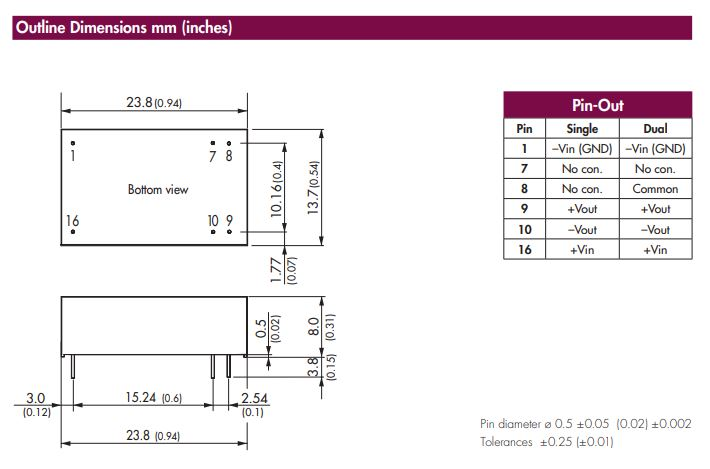
\includegraphics[scale=0.8]{convertidor_5vdc_datasheet}
  \caption{Dimensiones y pinout del convertidor TEL 2-0511 según su hoja de datos.}\label{fig:convertidor_5vdc_datasheet}
\end{figure}

\begin{figure}[!htb]
\minipage{0.4\textwidth}
  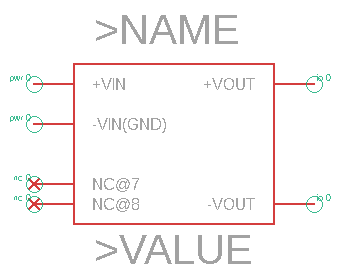
\includegraphics[width=\linewidth]{convertidor_5vdc_simbolo}
  \caption{Símbolo creado en Eagle del convertidor TEL 2-0511.}\label{fig:convertidor_5vdc_simbolo}
\endminipage\hfill
\minipage{0.4\textwidth}
  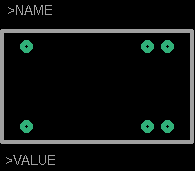
\includegraphics[width=\linewidth]{convertidor_5vdc_huella}
  \caption{Huella creada en Eagle del convertidor TEL 2-0511.}\label{fig:convertidor_5vdc_huella}
\endminipage\hfill
\end{figure}

\begin{figure}[!htb]
\centering
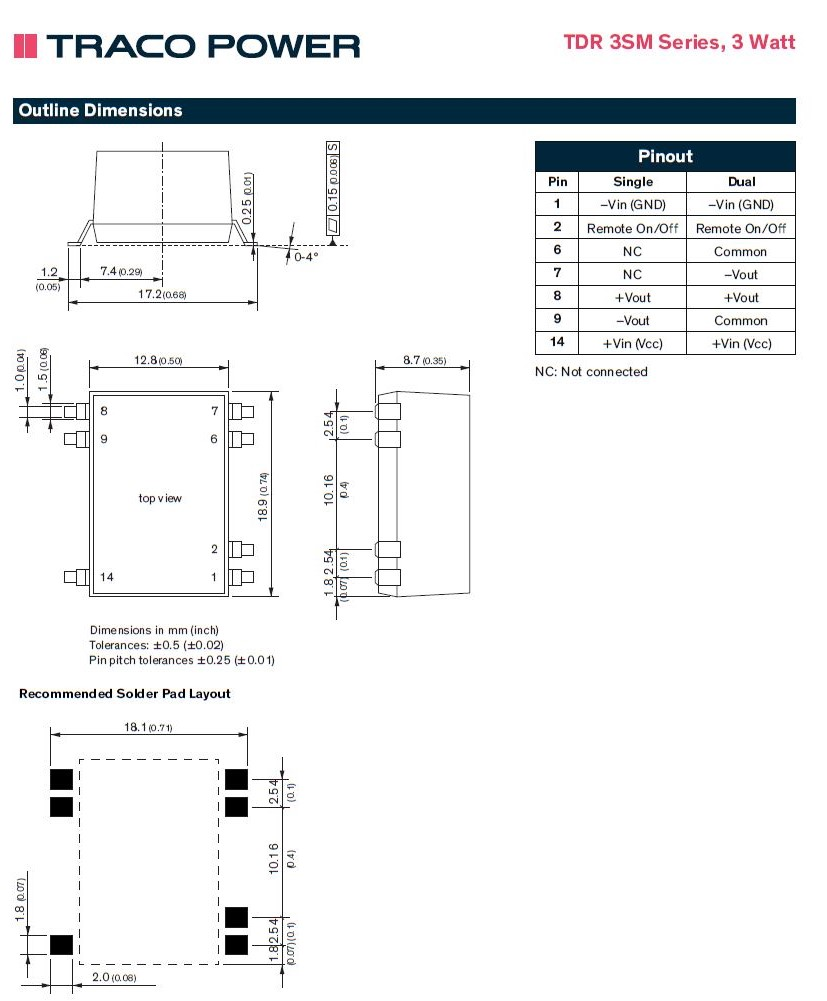
\includegraphics[scale=0.7]{convertidor_15vdc_datasheet}
  \caption{Dimensiones y pinout del convertidor TDR 3-0513SM según su hoja de datos.}\label{fig:convertidor_15vdc_datasheet}
\end{figure}

\begin{figure}[!htb]
\minipage{0.5\textwidth}
  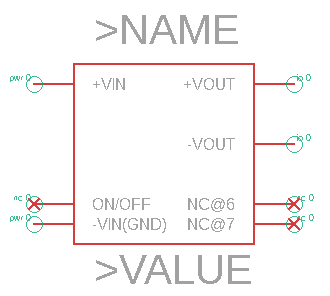
\includegraphics[width=\linewidth]{convertidor_15vdc_simbolo}
  \caption{Símbolo creado en Eagle del convertidor TDR 3-0513SM.}\label{fig:convertidor_15vdc_simbolo}
\endminipage\hfill
\minipage{0.3\textwidth}
  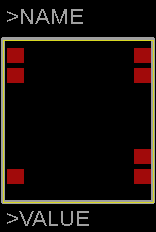
\includegraphics[width=\linewidth]{convertidor_15vdc_huella}
  \caption{Huella creada en Eagle del convertidor TDR 3-0513SM.}\label{fig:convertidor_15vdc_huella}
\endminipage\hfill
\end{figure}

Una vez se dispone de todos los componentes necesarios, se genera con ellos el esquemático de la etapa de potencia del mini TEREFES mostrado en la figura \ref{fig:pcb_potencia_esquematico}. Este diseño dispone únicamente de los componentes necesarios para la etapa de potencia del electroestimulador de la prótesis híbrida. Estos son, entrada de $5Vdc$ desde una batería externa, una fuente de $5Vdc$ y una fuente de $15Vdc$ y $\pm15Vdc$. Los puntos más importantes del esquemático son:

\begin{itemize}
\item[•] \textbf{Conector JP1:} entrada de $5Vdc$ desde la batería mediante este conector de cuatro pines, pues se conecta en serie un interruptor para poder cortar la alimentación y apagar el dispositivo.
\item[•] \textbf{Componentes U1, U2 y U3:} son los convertidores de corriente continua de $5Vdc$ a $5Vdc$, $5Vdc$ a $15Vdc$ y $5Vdc$ a $\pm15Vdc$ respectivamente.
\item[•] \textbf{Conectores JP2, JP3 y JP4:} Son los conectores que portan las salidas de los convertidores, es decir los niveles de tensión de $5Vdc$, $15Vdc$ y $\pm15Vdc$ y sus referencias a masa que necesita la tarjeta de control. Son estos los conectores que se desea alinear con los correspondientes de le placa de control en el montaje con los reversos enfrentados.
\item[•] \textbf{Conector JP5:} Este conector sirve para el control de encendido y apagado del convertidor U3. Si se desea encender el convertidor se ha de conectar el pin RC de U3 a su masa, es decir, -VIN la cual va a su vez conectada a la masa de la batería. Por el contrario, si se desea apagar el convertidor se ha de poner un nivel de tensión de $5Vdc$ en el pin RC. También se desea alinear este conector con su correspondiente punto en la placa de control.
\item[•] Se han añadido varios ``testpoints'' en los que poder medir fácilmente diferentes niveles de tensión, como la salida de los convertidores, una vez la placa esté fabricada y en funcionamiento.
\end{itemize}


\subsubsection{Tarjeta de circuito impreso}
Una vez finalizado el esquemático de la etapa de potencia del mini TEREFES, se genera ahora la distribución o ``layout'' de las huellas de todos sus componentes en la tarjeta de circuito impreso que los contendrá. 
\\
\\
Es un diseño sencillo por lo que dos capas son suficientes: la superior contiene todos los componentes y conexiones mientras que la inferior es el plano de masa de la batería y la conexión del pin RC del convertidor U3 al conector JP5. Además, para que la tarjeta disponga de conexiones a masa y señales robustas, se ha decidido utilizar polígonos en vez de pistas siguiendo el diseño de la tarjeta de potencia del TEREFES.
\\
\\
El punto más importante es la colocación de los conectores JP2, JP3 y JP4. Deben quedar alineados con los puntos correspondientes de la tarjeta de circuito impreso de la etapa de control. Para ello se han de tomar medidas sobre ésta y aplicarlas consecuentemente a los conectores mencionados. Se muestra entonces en la figura \ref{fig:pcb_control_layout} del Anexo I el anverso de la placa de control con las medidas mencionadas. Ahora, para la colocación de los conectores JP2, JP3 y JP4 en la placa de potencia se ha de considerar la imagen especular de los conectores correspondientes de la placa de control según uno de los lados verticales. Esto es lo miso que lo ya explicado en la figura \ref{fig:montaje_alineado}. Se muestra en la figura \ref{fig:pcb_potencia_layout} la distribución de los componentes de la tarjeta de la etapa de control. Sin embargo, se puede ver que las medidas verticales tomadas sobre las placas de potencia y control no coinciden, las de la tarjeta de potencia son $1mm$ más largas. Los conectores de ambas placas están alineados, pero se ha hecho la placa de potencia $1mm$ más larga. Esto es así para que los polígonos que utilizan los conectores JP3 y JP4 los rodeen totalmente y la conexión eléctrica sea robusta.
\\
\\
Se pueden apreciar también en el Anexo II la capa superior, inferior y el modelo de fabricación de la tarjeta de potencia en las figuras \ref{fig:pcb_potencia_top}, \ref{fig:pcb_potencia_bottom} y \ref{fig:pcb_potencia_modelo} respectivamente.\\

\subsection{Validación de objetivos}


\section{Etapa de control}
La etapa de control es mucho más robusta que la de potencia. Sin embargo, existen vías de mejora cuya implementación se explica en este apartado.

\subsection{Revisión del hardware y planteamiento de objetivos de mejora}
Se ha mencionado con anterioridad que la tarjeta de la etapa de potencia tiene un convertidor de corriente continua de $5Vdc$ a $\pm15Vdc$. Este convertidor dispone de una entrada denominada RC o ``Remote Control'' que según su hoja de datos controla el encendido y apagado del mismo. Esto permite que en su salida haya $\pm15Vdc$ o $0Vdc$. En el diseño original de la etapa de potencia del estimulador se hace este tipo de control, lo cual se mantiene tras mejorar el hardware de dicha etapa según el apartado \ref{mejora_hardware_potencia}. Esta funcionalidad permite reducir el consumo del electroestimulador mientras esté encendido pero no utilizándose para aportar asistencia al paciente.
\\
\\
Para llevar a cabo el control remoto del convertidor de $\pm15Vdc$ se ha de manejar el nivel de tensión en su entrada RC. Si se desea apagar el convertidor, esta entrada debe estar a $5Vdc$. Si por el contrario, se desea encenderlo, RC debe estar conectada a la masa del convertidor. Es el microcontrolador ATmega128L de la etapa de control el que efectúa el encendido y apagado. Para ello, se sirve del puerto G1 conectado a RC mediante uno de los dos pines de la conexión 2 de la figura \ref{fig:pcb_control_layout}. Esta conexión es una de las que se ha discutido en la mejora del hardware de la etapa de potencia, pues queda alineada en el montaje de reversos enfrentados con su correspondiente punto en la placa de dicha etapa. Se aprecia la conexión descrita en las figuras \ref{fig:RC_convertidor_control} y \ref{fig:RC_convertidor_potencia}.\\

\begin{figure}[!htb]
\minipage{0.45\textwidth}
  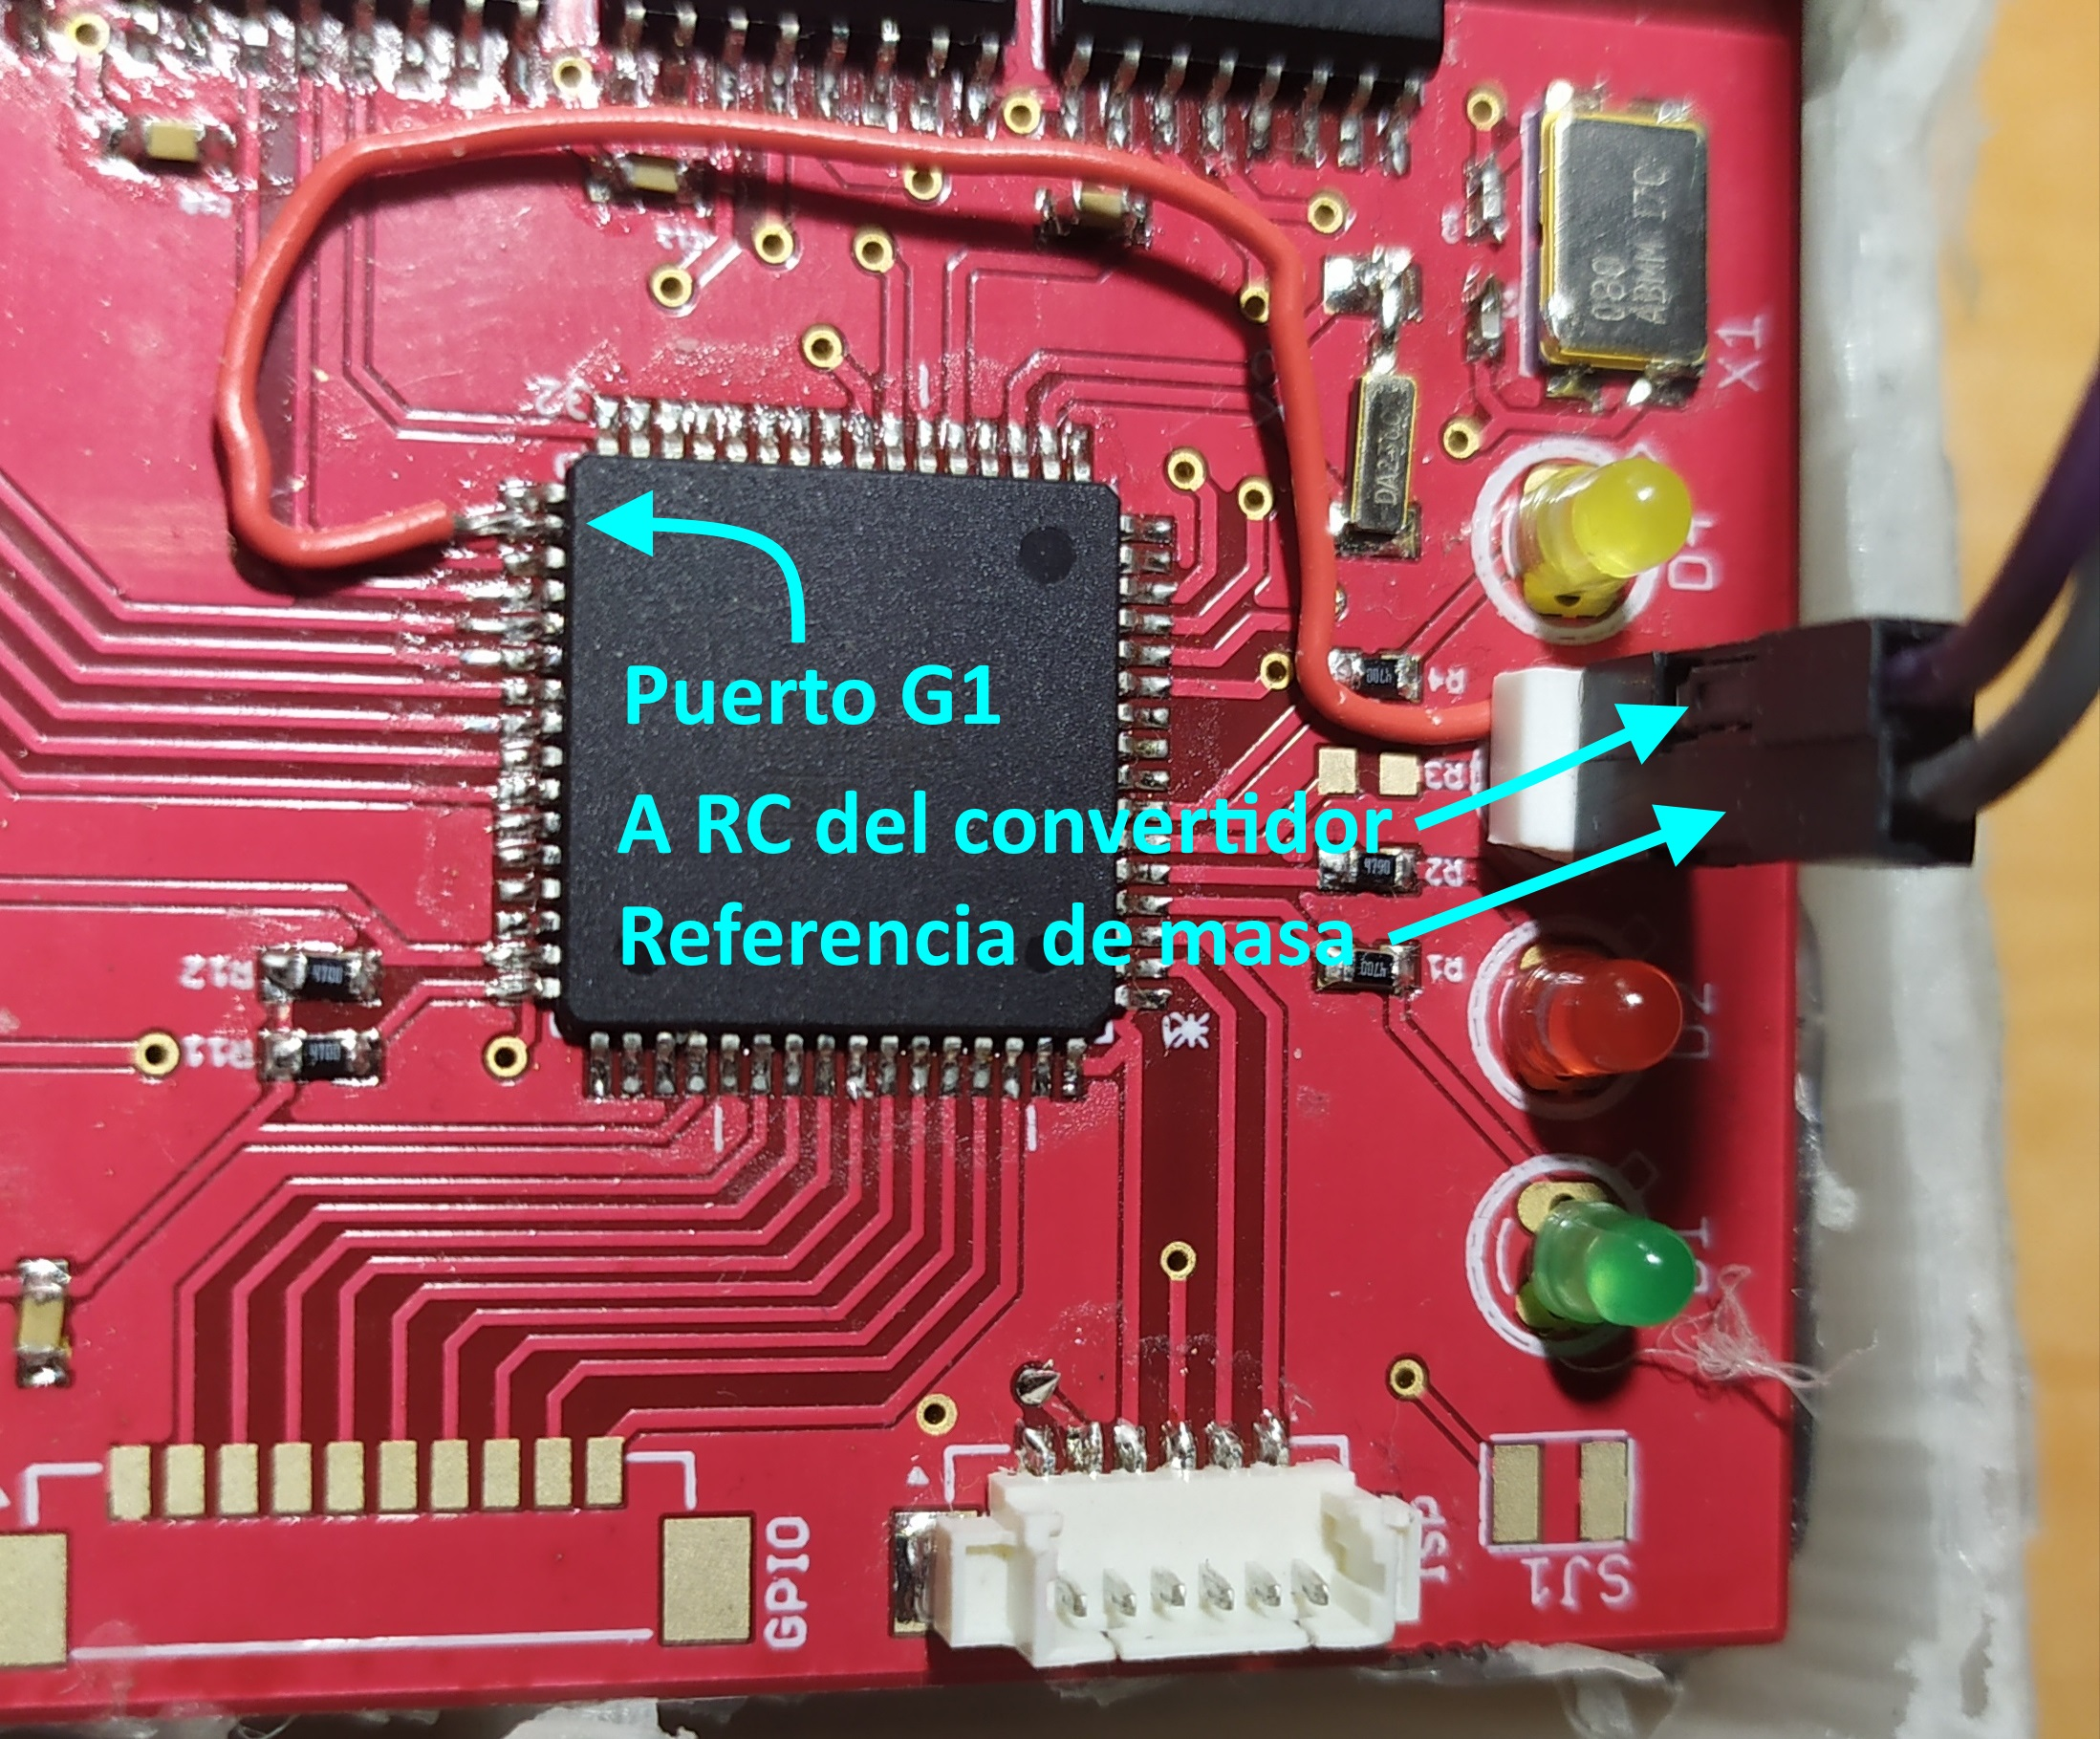
\includegraphics[width=\linewidth]{RC_convertidor_control}
  \caption{Conexión del microcontrolador a un pin montado en la placa de control. Este pin se conecta a su vez con un jumper a la entrada RC del convertidor de $5Vdc$ a $\pm15Vdc$ en la tarjeta de potencia.}\label{fig:RC_convertidor_control}
\endminipage\hfill
\minipage{0.45\textwidth}
  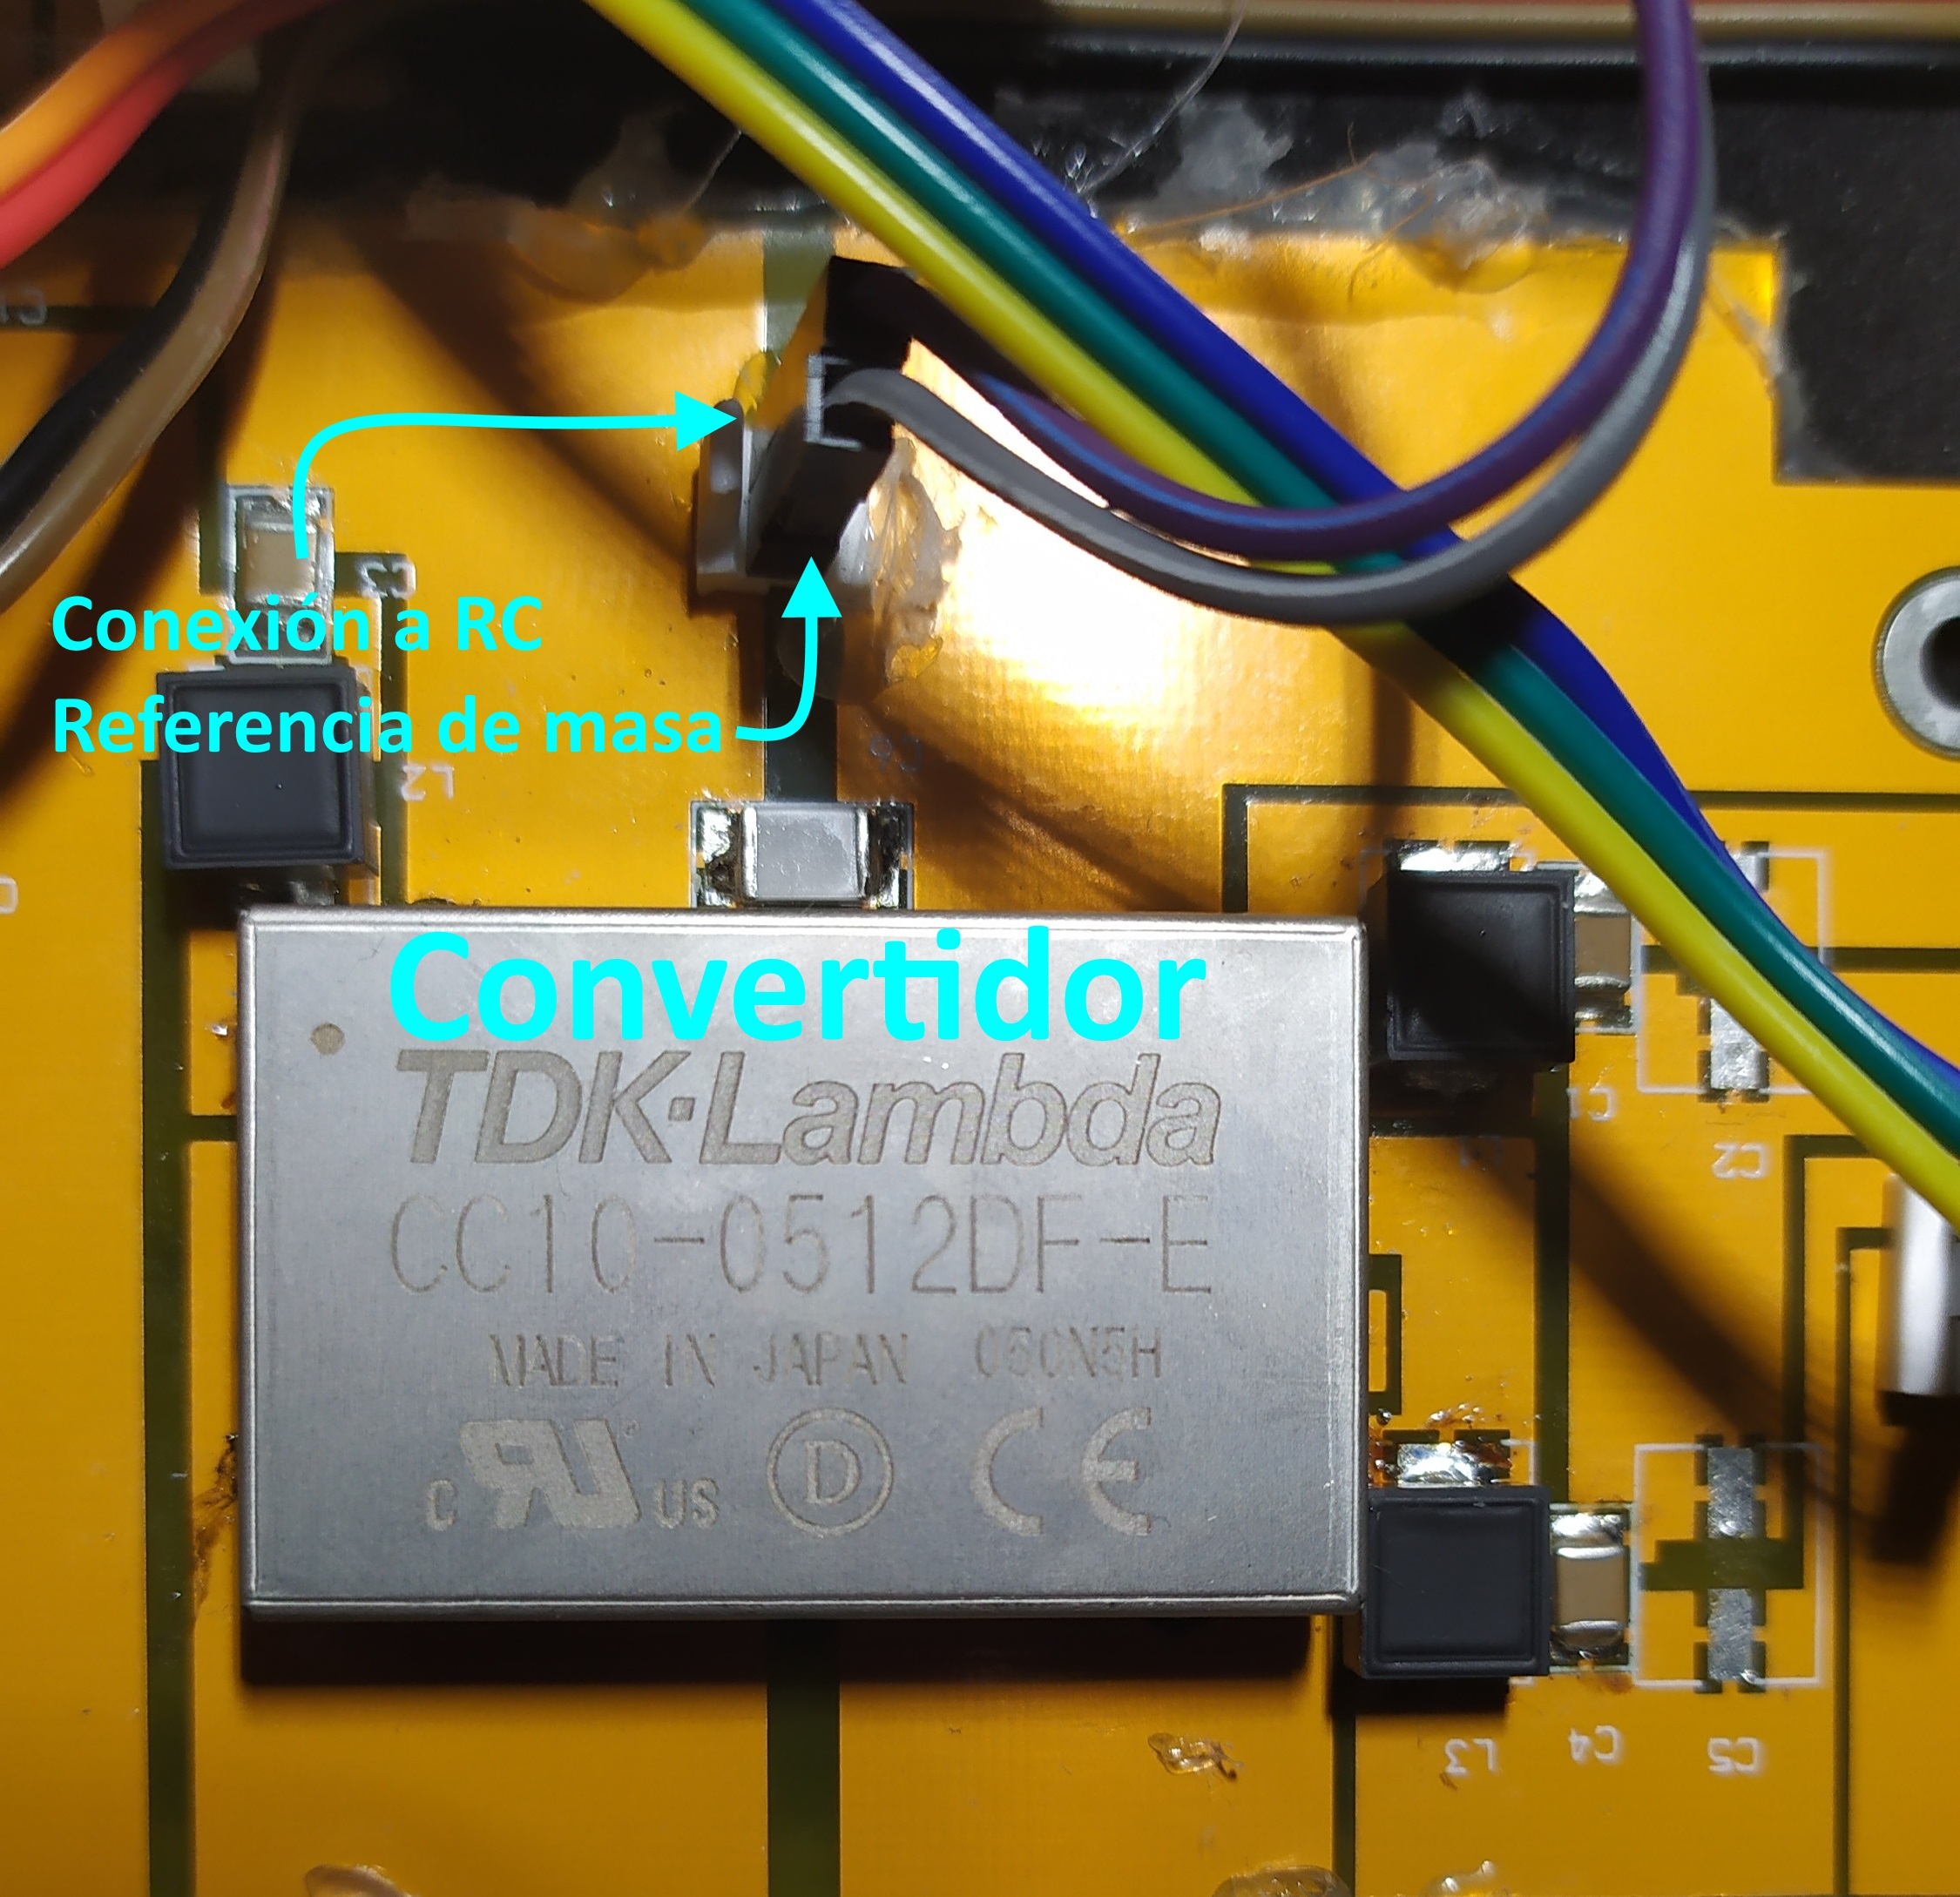
\includegraphics[width=\linewidth]{RC_convertidor_potencia}
  \caption{Conexión para el control remoto del convertidor de $5Vdc$ a $\pm15Vdc$ mediante un cable desde la etapa de control.}\label{fig:RC_convertidor_potencia}
\endminipage\hfill
\end{figure}

Se puede ver en la figura \ref{fig:RC_convertidor_control} cómo un cable rojo une el puerto G1 del microcontrolador con el pin situado entre los leds amarillo y rojo. Esto es un punto débil en la etapa de control ya que esta conexión no es óptima en términos eléctricos ni mecánicos. Esto se explica porque la soldadura puede no ser correcta al formarse un puente con los pines colindantes del microcontrolador o el cable puede presentar problemas. Se plantea entonces una alternativa para sustituir esta conexión por otra implementada de una forma más robusta y fiable sin tener que rediseñar la tarjeta de circuito impreso. Para ello, se tomará ventaja del hecho de que la placa de control también está diseñada para el estimulador TEREFES, el cual tiene dos fuentes de $15Vdc$ y $\pm15Vdc$. Esto permite el uso de una de las pistas de la tarjeta de control que no se ha utilizado ya que se empleaba para una de la fuentes de tensión del TEREFES que no tiene el mini TEREFES.

\subsection{Tareas para la mejora del hardware}
Se puede ver en la figura \ref{fig:pcb_control_layout} del Anexo I, junto a la conexión 2, otras tres conexiones denominadas D1, D2 y D4. Se pueden ver más fácilmente dichas conexiones en la parte inferior izquierda de la imagen representativa de la placa en el Anexo I. En estas conexiones se sitúan tres leds los cuales indican si la estimulación eléctrica está activa, si el convertidor de $5Vdc$ a $\pm15Vdc$ está encendido y si el estimulador está encendido, respectivamente. Sin embargo, D3, es decir la conexión 2, se utiliza para el control remoto del convertidor tal y como ya se ha explicado.
\\
\\
Cuando esta tarjeta de circuito impreso se utilizaba en el TERFES, en la conexión 2 había un led que indicaba el estado del segundo convertidor de $5Vdc$ a $\pm15Vdc$. Sin embargo, en el mini TEREFES no se utiliza la pista que une el alojamiento de dicho led con el puerto E4 del microcontrolador, el cual lo enciende o apaga.
\\
\\
Lo que se propone es prescindir del cable que une el puerto G1 del microcontrolador con el pin que lleva al control remoto del convertidor. A continuación, se desea implementar el control remoto mediante el puerto E4 que está unido con una pista al alojamiento D3 o lo que es lo mismo, la conexión 2 mencionada previamente. En éste se encuentran los pines que se conectan al RC del convertidor y su referencia a masa de la forma explicada en el apartado de mejora del hardware de la etapa de potencia. Se expone con más detalle este procedimiento en la figura \ref{fig:mejora_RC}. En esta figura se aprecia que la unión azul, la de la pista en la tarjeta de circuito impreso, está dividida por dos cuadros naranjas. Éstos representan la huella de la resistencia originalmente une el puerto del microcontrolador con el pin RC. La resistencia era necesaria cuando en esta conexión se alojaba el led que indicaba el estado del segundo convertidor del TEREFES. En el caso del mini TEREFES no es necesario utilizarla por lo que la pista se cierra utilizando una resistencia de $0\Omega$.\\

\begin{figure}[!htb]
\centering
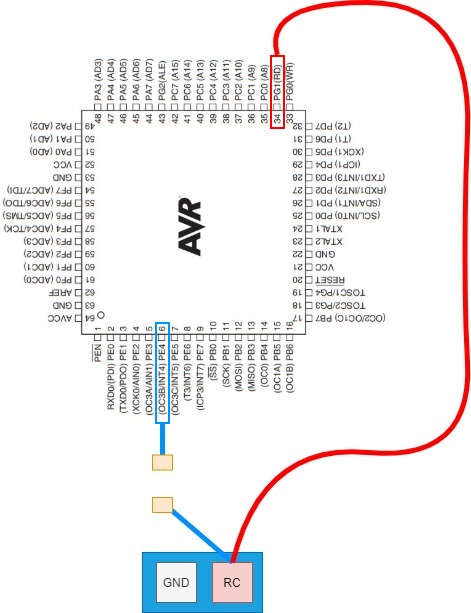
\includegraphics[scale=0.7]{mejora_RC}
  \caption{Representación del control del convertidor desde el microcontrolador. La unión roja es el cable del que se desea prescindir mientras que la unión azul es la pista de la tarjeta de circuito impreso que se va a utilizar. El rectángulo azul representa la conexión 2 de la figura \ref{fig:pcb_control_layout} que contiene los pines que se conectan a la referencia de masa y RC del convertidor que se desea controlar.}\label{fig:mejora_RC}
\end{figure}

Esta tarea de mejora conlleva inevitablemente modificar el firmware del electroestimulador. Esto se debe a que el control remoto del convertidor de $5Vdc$ a $\pm15Vdc$ se hace ahora mediante el puerto E4 y no el G1. Se muestran a continuación las líneas de código que se encargan del control remoto del convertidor mediante el puerto G1:

\begin{lstlisting}[language=C++,breaklines]
case CMD_ON1:	//se desea encender la fuente 
	PORTG &= ~(1<<PORTG1);	//Encender fuente, 0Vdc a RC mediante PG1
	PORTE |= (1<<PORTE3);	//Encender led de estado de fuente
	
case CMD_OFF1:	//se desea apagar la fuente 
	PORTG |= (1<<PORTG1);	//Apagar fuente, 5Vdc a RC mediante PG1
	PORTE &= ~(1<<PORTE3);	//Apagar led de estado de fuente
\end{lstlisting}

Estas líneas se modifican para hacer uso del puerto E4:

\begin{lstlisting}[language=C++,breaklines]
case CMD_ON1:	//se desea encender la fuente 
	PORTE &= ~(1<<PORTE4);	//Encender fuente, 0Vdc a RC mediante PE4
	PORTE |= (1<<PORTE3);	//Encender led de estado de fuente
	
case CMD_OFF1:	//se desea apagar la fuente 
	PORTE |= (1<<PORTE4);	//Apagar fuente, 5Vdc a RC mediante PE4
	PORTE &= ~(1<<PORTE3);	//Apagar led de estado de fuente
\end{lstlisting}

Se puede ver que se hace uso de un ``switch case'' para la interpretación de tareas en el microcontrolador según el comando indicado. Para el caso los comandos son CMD\_ON1 y CMD\_OFF1 para encender y apagar el convertidor, respectivamente. 
\\
\\
Para que el uso del PE4 sea efectivo, se ha de establecer el valor correcto en el registro de direcciones del puerto E del microcontrolador. De este modo, el puerto E4 debe estar configurado como salida por lo que el bit 3 del registro DDRE debe contener un valor de 1 tal y como se indica a continuación:

\begin{lstlisting}[language=C++,breaklines]
DDRE |= ((1<<DDE2) | (1<<DDE3) | (1<<DDE4) | (1<<DDE5) | (1<<DDE6) | (1<<DDE7));
\end{lstlisting}
\subsection{Validación de objetivos}
Según las tareas descritas en el apartado anterior, se ha eliminado el cable que une el puerto G1 del microcontrolador con el pin que conecta al control remoto del convertidor. Además, se ha cerrado la pista de la tarjeta de control con una resistencia de $0\Omega$. De este modo, es ahora el puerto E4 del ATmega128L el que controla el encendido y apagado del convertidor de $\pm15Vdc$ tal y como se deseaba. Se aprecia en la figura \ref{fig:mejora_RC_terminado} la mejora efectuada en el hardware, así como su validación en la figura \ref{fig:mejora_RC_terminado} que muestra la fuente de tensión encendida tras esta mejora.\\

\begin{figure}[!htb]
\minipage{0.45\textwidth}
  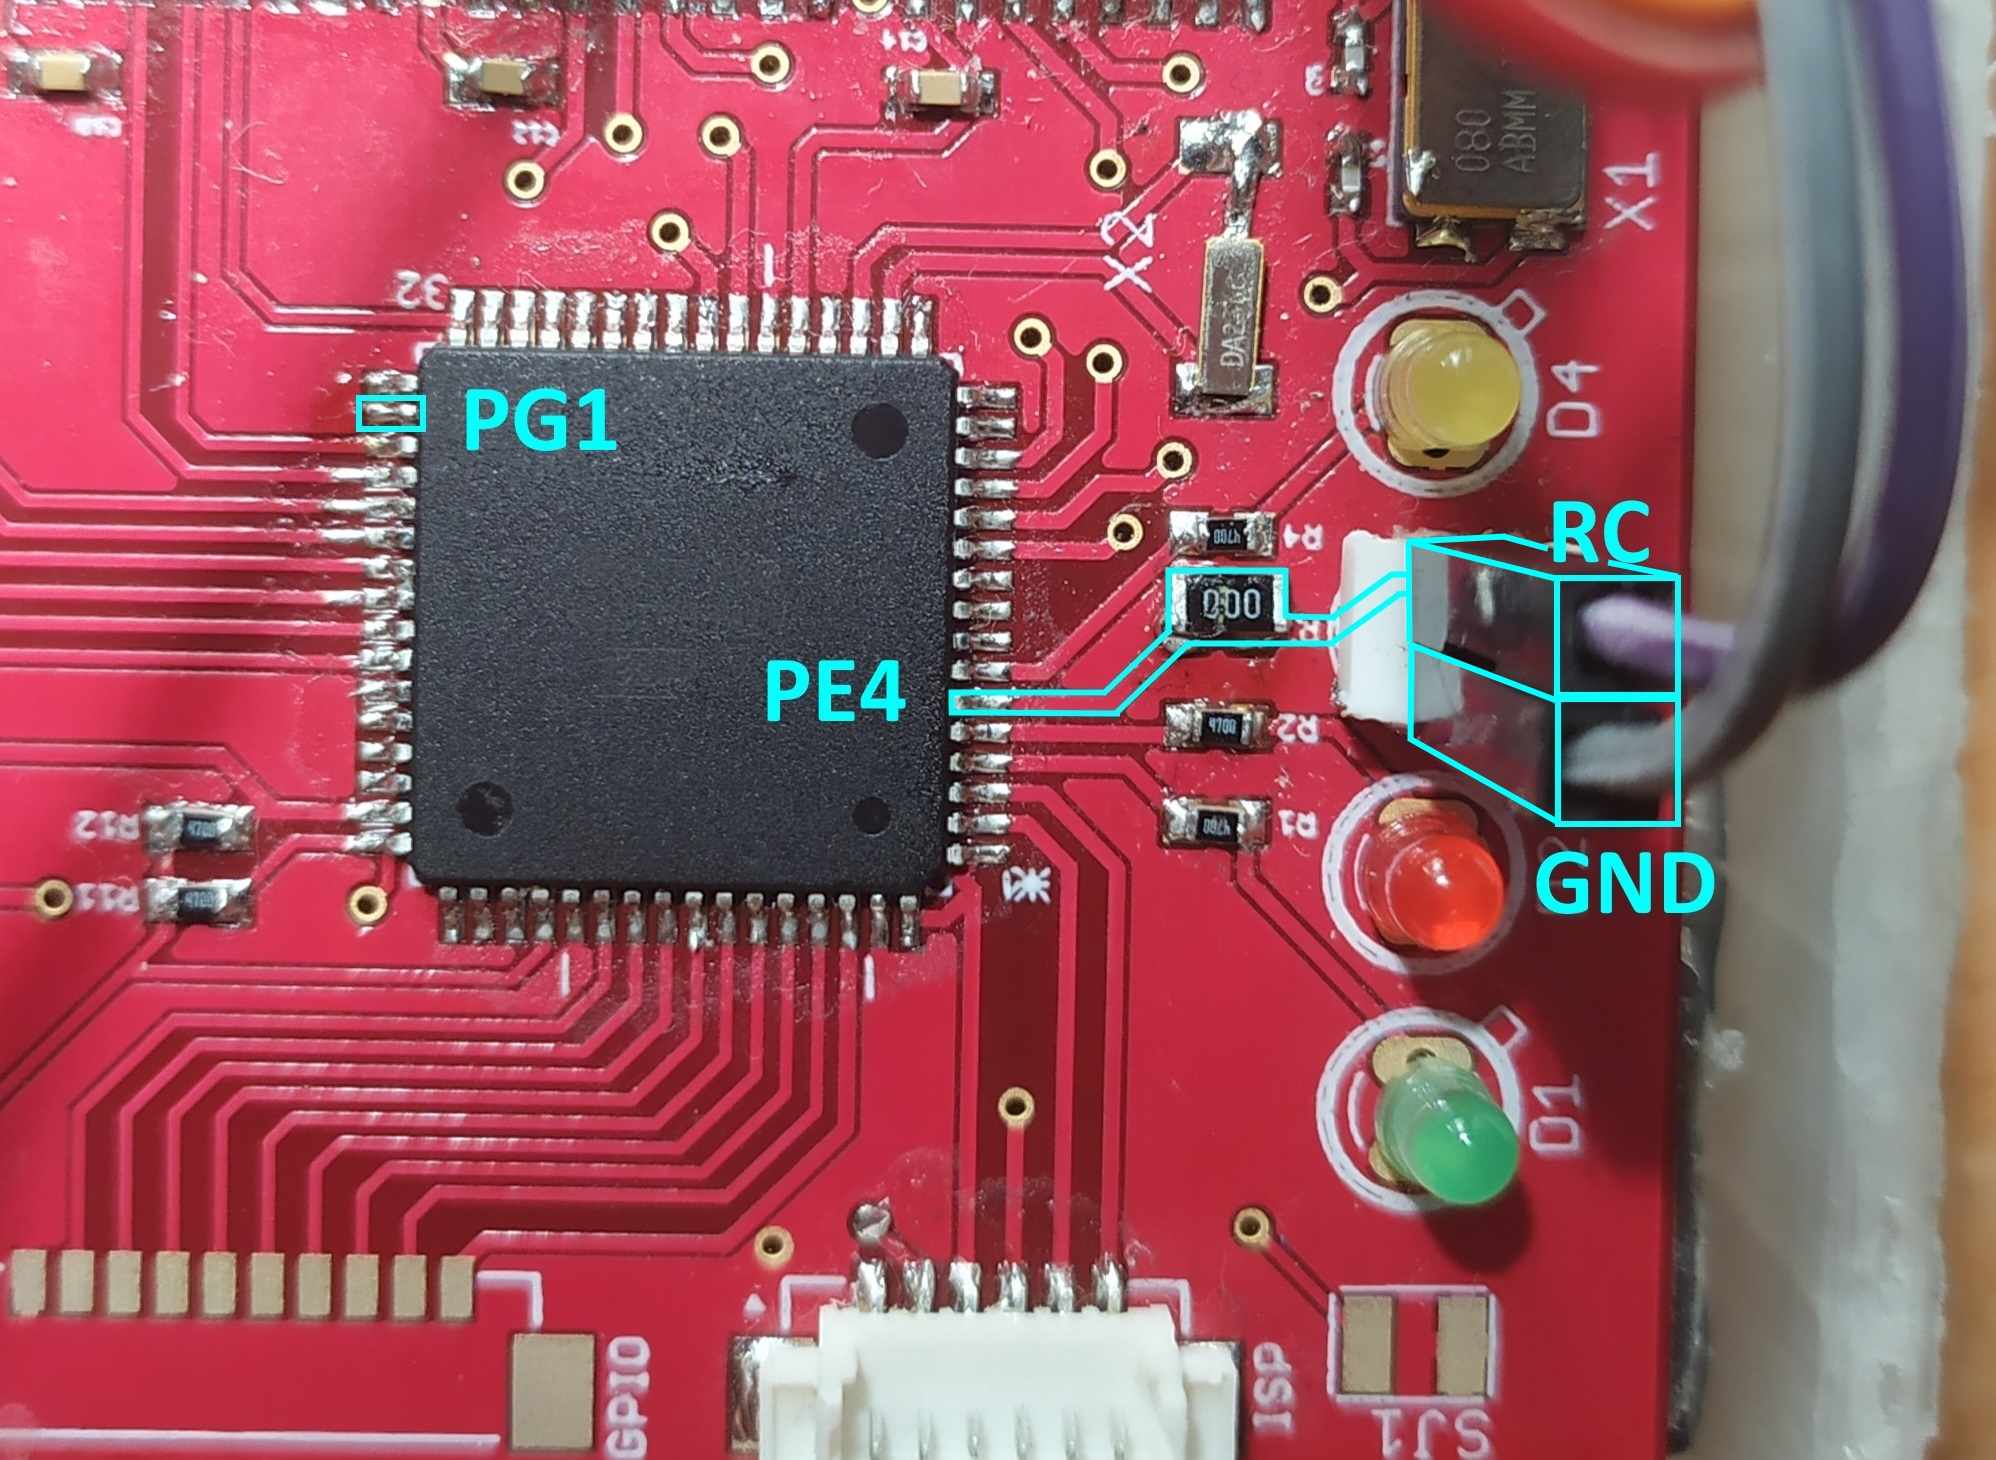
\includegraphics[width=\linewidth]{mejora_RC_terminado}
  \caption{Tarjeta de control tras la mejora del hardware para el control remoto del convertidor de $\pm15Vdc$. Se aprecia que ya no hay ningún cable soldado al PG1 así como hay una resistencia de $0\Omega$ en la pista señalada en azul, junto al PE4.}\label{fig:mejora_RC_terminado}
\endminipage\hfill
\minipage{0.45\textwidth}
  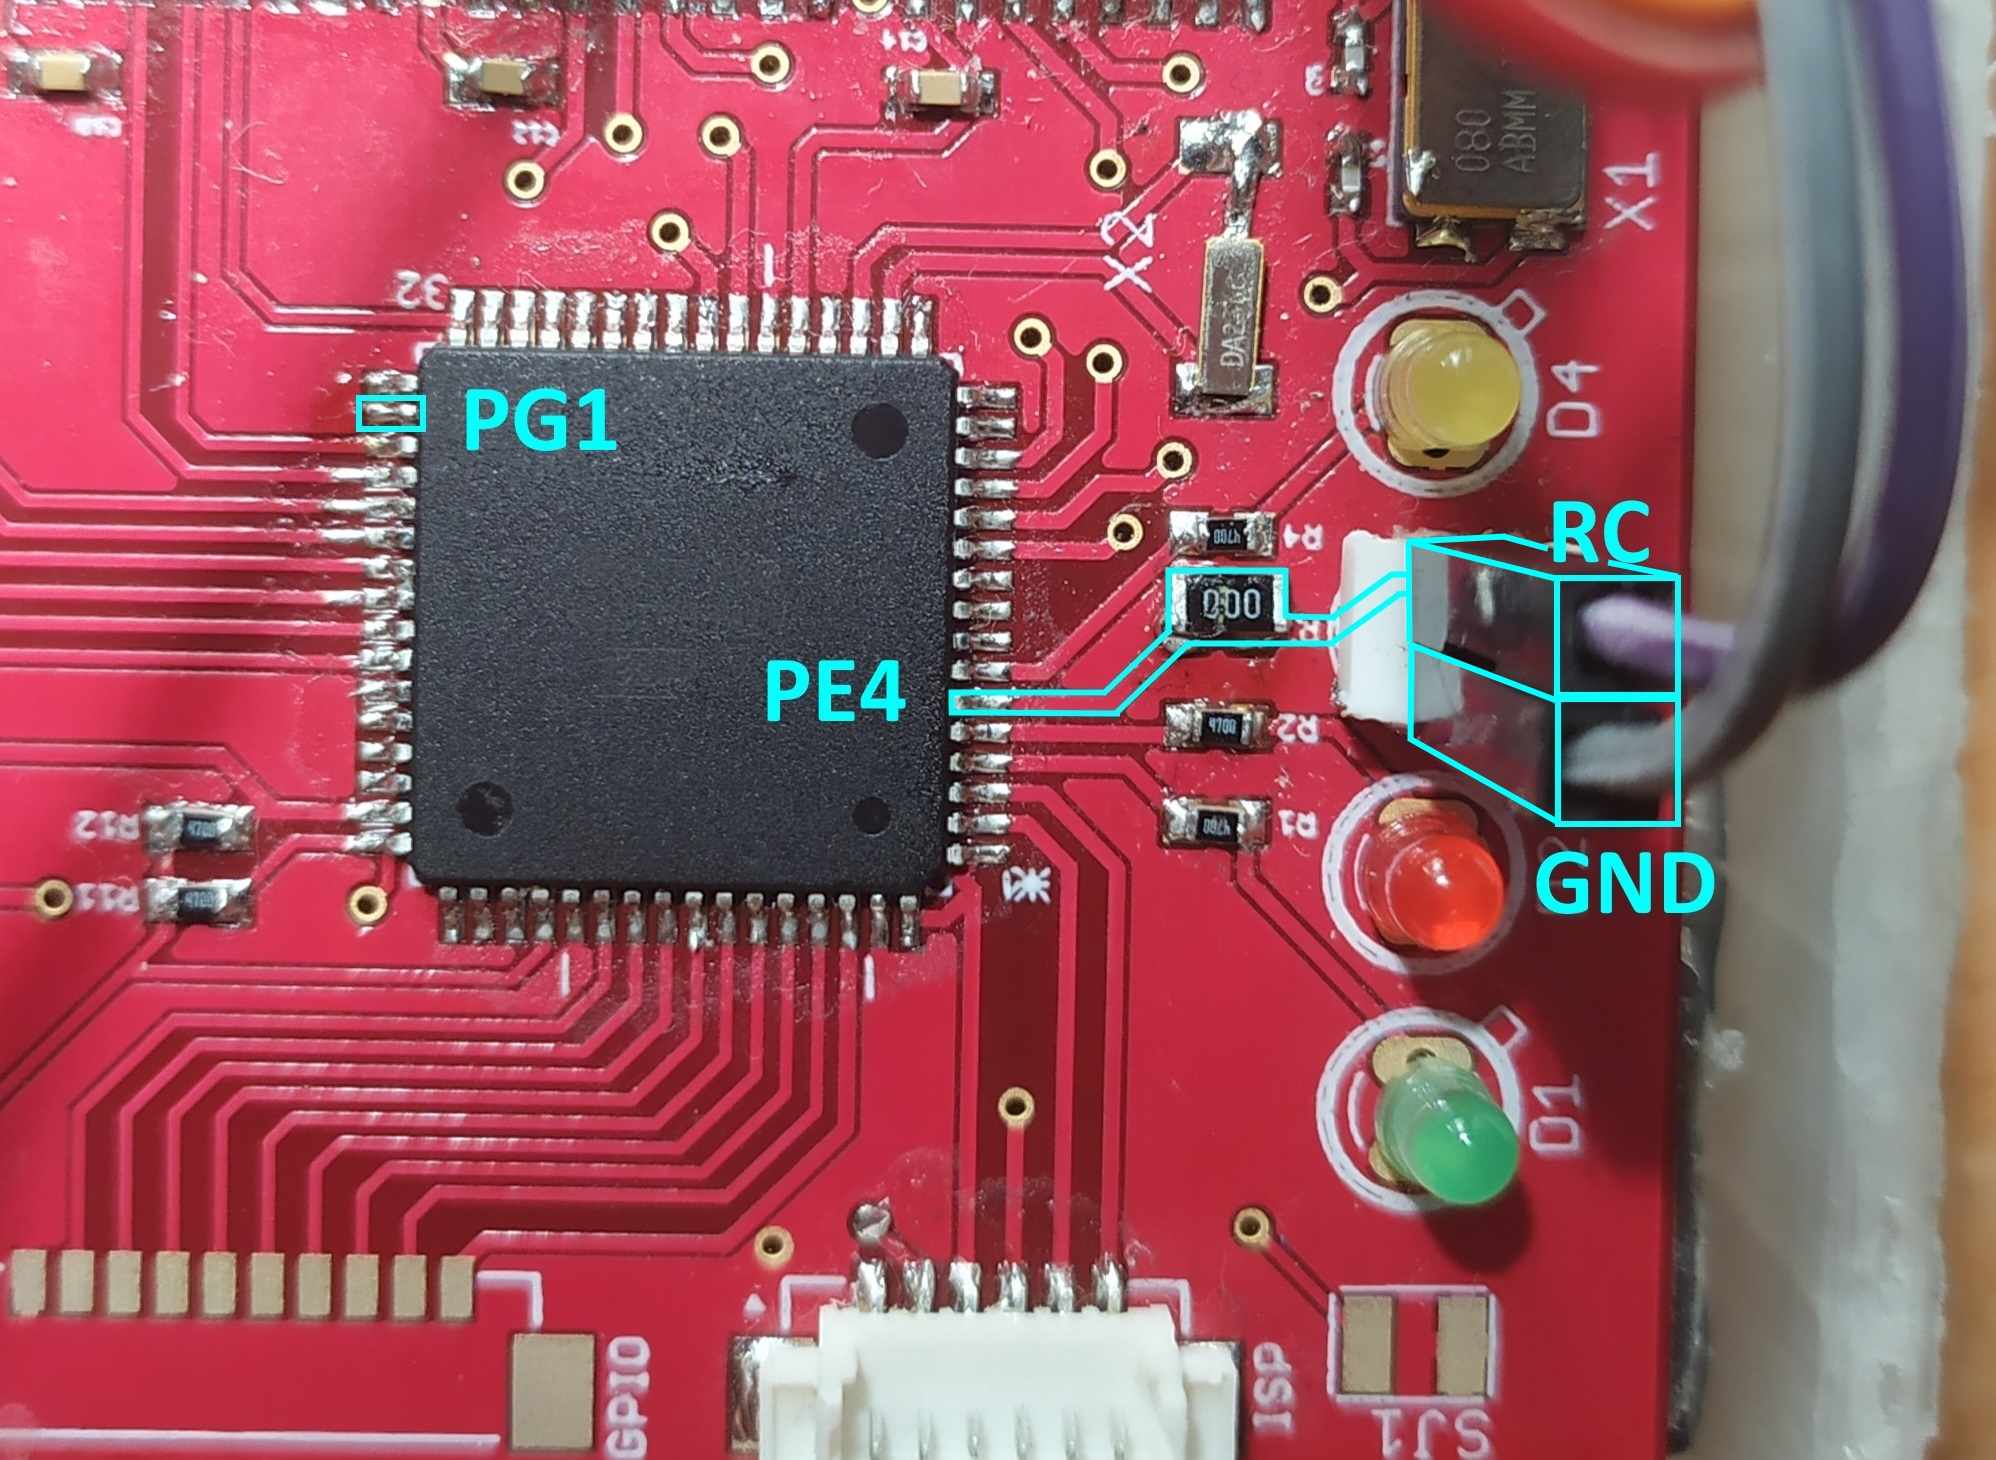
\includegraphics[width=\linewidth]{mejora_RC_terminado}\caption{Medición en la salida del convertidor de $\pm15Vdc$. El convertidor se ha encendido mediante el control remoto haciendo uso del PE4 del microcontrolador.}\label{fig:mejora_RC_terminado}
\endminipage\hfill
\end{figure}

